%
\hsection{Pip and Virtual Environments}%
%
The go-to tool for installing \python\ packages is \pip.
The standard way to install packages for use with \python\ is in a so-called virtual environment.
%
\hsection{Pip and Virtual Environments in \ubuntu\ \linux}%
%
\begin{figure}%
\centering%
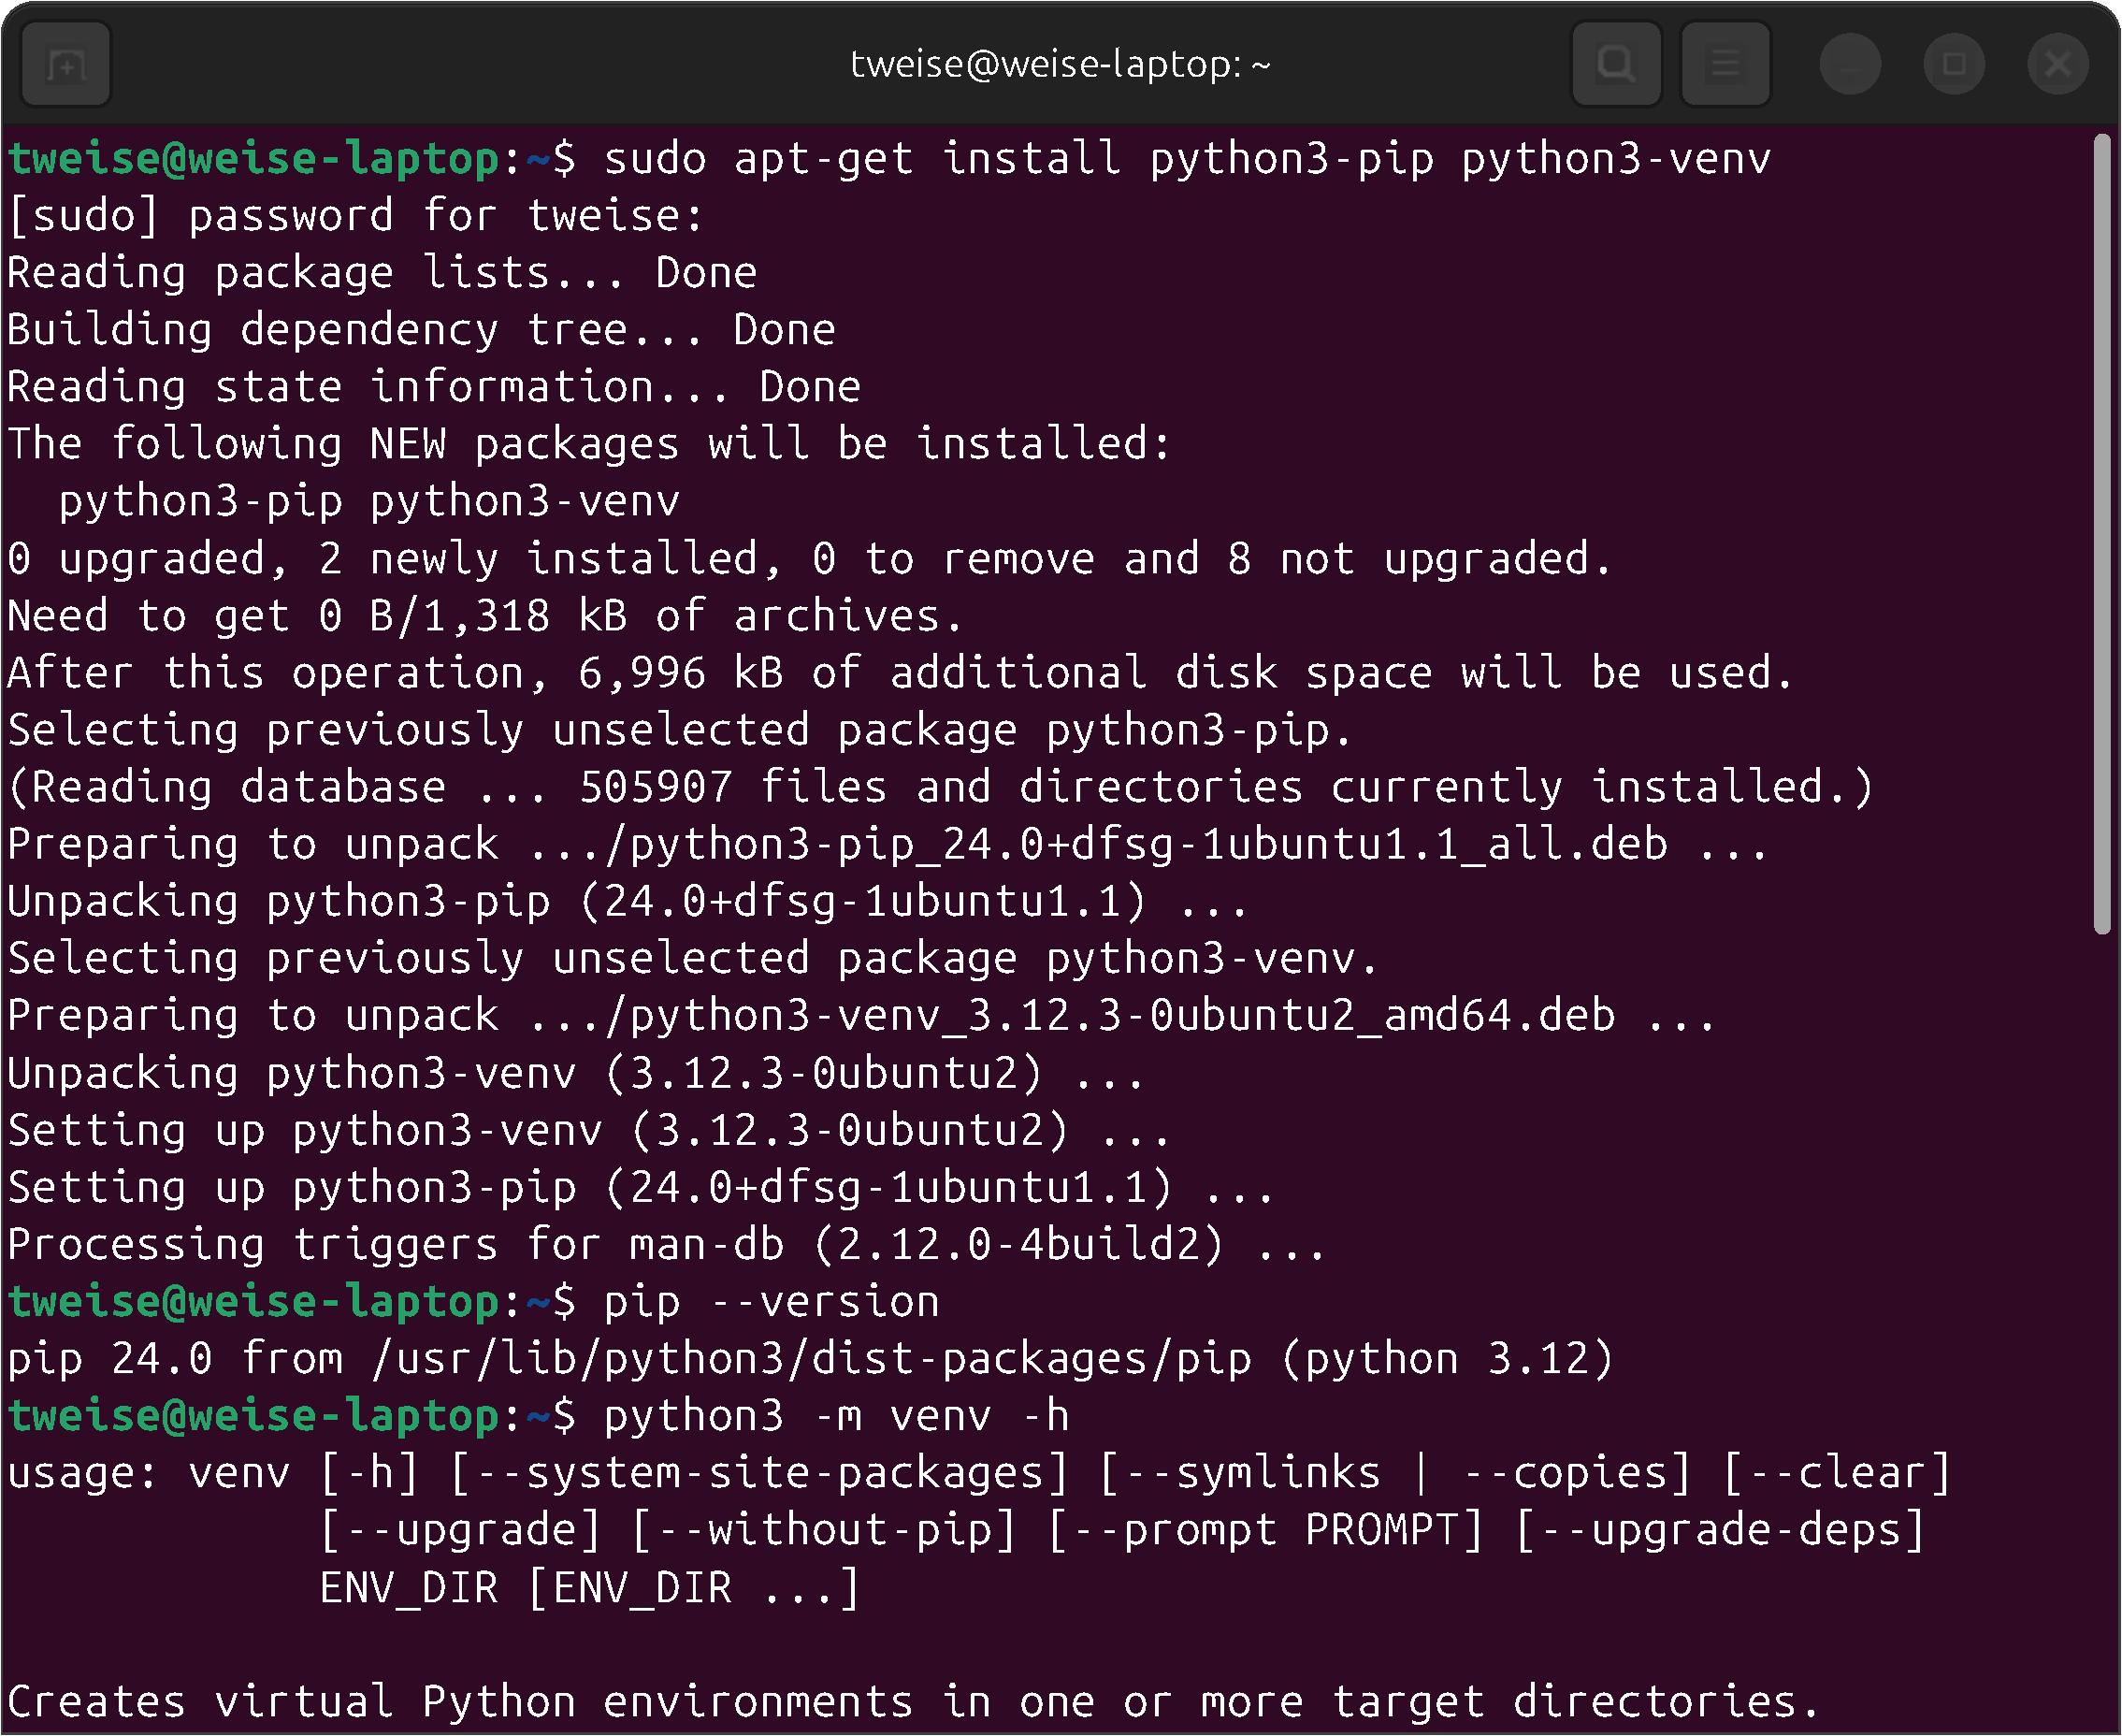
\includegraphics[width=0.7\linewidth]{\currentDir/installPipVenvUbuntu}%
\caption{Installing \pip\ and venv under \ubuntu\ \linux: \pip~is usually already installed, venv not. %
We need to use the \bashil{apt-get} route to make sure that both \bashil{python3-pip} and \bashil{python3-venv} are installed.}%
\label{fig:installPipVenvUbuntu}%
\end{figure}%
%
\gitBashAndOutput{\programmingWithPythonCodeRepo}{10_packages}{numpy_user_venv.sh}{packages:numpy_user_venv}{%
An example of using virtual environments and \pip\ under \ubuntu\ \linux.}%
%
\endhsection%
%
\hsection{Pip and Virtual Environments under \windows}%
%
\begin{figure}%
\centering%
\tightbox{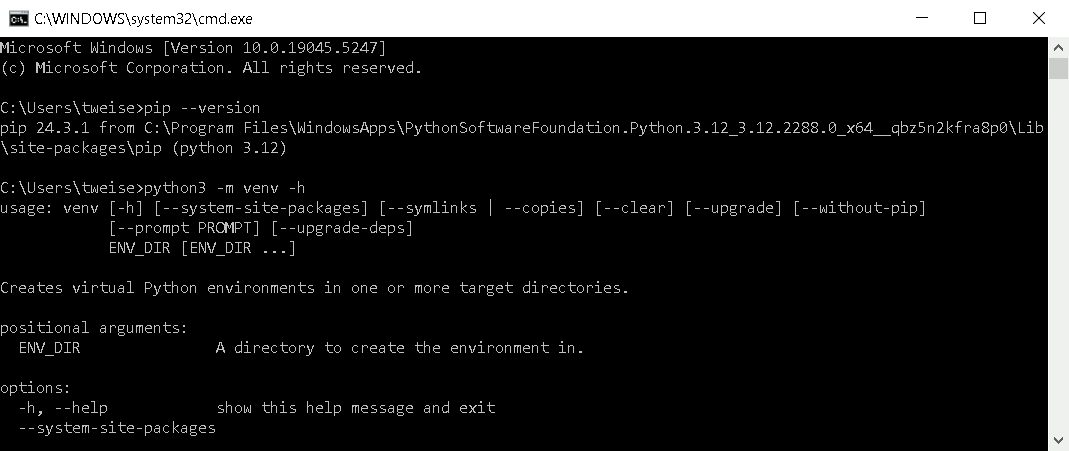
\includegraphics[width=0.85\linewidth]{\currentDir/installPipVenvWindows}}%
\caption{Installing \pip\ and venv under \windows: They are already installed.}%
\label{fig:installPipVenvWindows}%
\end{figure}%
\endhsection%
%
\FloatBarrier%
\endhsection%
%
